\chapter{Related Work}
\label{chap:related}

This chapter will showcase similar or relevant research to this thesis.
Section \ref{sec:starcoder} will show Starcoderdata, a dataset used by various code synthesis models for training or further data extraction.
Section \ref{sec:synthmodels} will show other models trained for code synthesis and their approach to dataset creation, architecture and training.

\section{Starcoderdata}
\label{sec:starcoder}
The Starcoderdata dataset\footnote{\url{https://huggingface.co/datasets/bigcode/Starcoderdata} (last visited on 2024-10-31)} is the dataset used for training the StarCoder code synthesis model.
Both were introduced by Li et al. \cite{Li.2023} as part of the BigCode umbrella, like The Stack dataset.
In fact, Starcoderdata is derived from The Stack (v1.2), which was introduced in section \ref{sec:thestack}.
To create Starcoderdata, Li et al. first chose all languages with over 500 MB of data, as well as the top 50 popular languages on GitHub as of December 2022\footnote{\url{https://web.archive.org/web/20221229040526/https://www.tiobe.com/tiobe-index/} (last visited on 2024-10-31)}, excluding unsupported and configuration languages, and including dialects of selected languages.
They then apply many -- often language- or language group-specific -- filters to their data, such as excluding files that begin with an XML header or files that have less than 25\% alphabetic characters.
This first pass gives them 815 GB of data, or close to 306 million files of code.

Next, they individually process all Jupyter Notebooks, GitHub issues and Git commits, and then deduplicate the dataset.
To deduplicate, they follow Allal et al.'s pipeline \cite{Allal.2023}.
They apply this pipeline to everything except for GitHub issues and Git commits.
Finally, they re-weigh JSON and YAML to 1 GB and CSS to 3 GB, arguing that all other languages are properly represented and balanced.
This results in the Starcoderdata dataset, with 207 M rows of data.


\section{Code Synthesis Models}
\label{sec:synthmodels}

This section will showcase code synthesis models introduced in other works, exploring how and on what data they have been trained and how well they perform.
This list is by no means exhaustive, as training code models is very popular at the moment (CodeLlama \cite{Roziere.2023}, CodeQwen \cite{Bai.2023}, WaveCoder \cite{Yu.2024} and many more are listed on the EvalPlus leaderboard\footnote{\url{https://evalplus.github.io/leaderboard.html} (last visited on 2024-10-31)} alone).


\subsection{WizardCoder}
\label{sec:wizardcoder}
WizardCoder, developed by Luo et al. \cite{Luo.2024}, is a code synthesis model trained with WizardLM's Evol-Instruct approach \cite{Xu.2024}.
It was fine-tuned from StarCoder, the model originally trained on Starcoderdata.

Evol-Instruct (as in Evolution) takes predefined instructions for training \acp{lm} and generates more instructions by prompting another \ac{lm} with the original instruction and a prompt template to evolve it based on certain metrics.
Luo et al. adapt this method for coding with the prompt template shown in fig \ref{fig:evolinst}, where \texttt{\{question\}} is a code question to be evolved and \texttt{\{method\}} consists of five methods, such as providing buggy code or adding ten additional words.

\begin{figure}[!h]
    \centering
    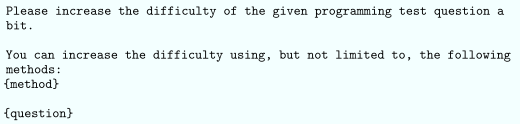
\includegraphics[width=\textwidth]{bilder/kapitel3/evolinst.png}
    \caption{The Evol-Instruct prompt template from \cite{Luo.2024}.}
    \label{fig:evolinst}
\end{figure}

They apply this template to 20.000 samples of the CodeAlpaca dataset\footnote{\url{https://huggingface.co/datasets/theblackcat102/evol-codealpaca-v1} (last visited on 2024-10-31)} to generate their training dataset.
They train iteratively, applying evol-instruct for every epoch and evaluating on HumanEval until they see a decline in pass@1.

At the time of release, WizardCoder was the most prolific open-source code synthesis model, reaching 57\% on HumanEval and 52\% on MBPP, as well as between 33\% and 55\% on DS-1000.


\subsection{Magicoder}
\label{sec:magicoder}
The Magicoder series, introduced by Wei et al. \cite{Wei.2024}, comprise four models trained with the OSS-Instruct approach also first introduced by them.
OSS-Instruct works as follows:
First, a set of seed code snippets is chosen. Wei et al. use Starcoderdata as a base and select 80.000 seed snippets, 40.000 from Python and 5.000 each from C++, Java, TypeScript, Shell, C\#, Rust, PHP and Swift.
A seed snippet in this case refers to 1-15 consecutive lines extracted from a random position in a file of the dataset.
Each seed snippet comes from a different file.
The seed snippets are then applied to the prompt shown in figure \ref{fig:magicoder}.
The prompt in sent to a teacher model, in their case gpt-3.5-turbo-1106, which responds with a problem and a solution.

\begin{figure}[!h]
    \centering
    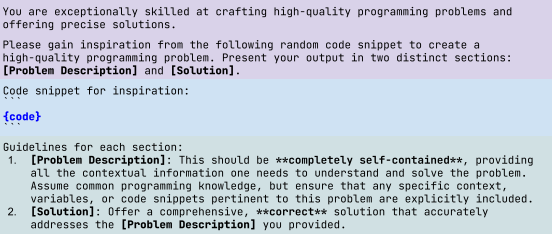
\includegraphics[width=\textwidth]{bilder/kapitel3/magicoder.png}
    \caption{The OSS-Instruct prompt template from \cite{Wei.2024}.}
    \label{fig:magicoder}
\end{figure}

Next, extensive data decontamination is done, disgarding samples that are identical, as well as removing samples containing docstrings, prompts, questions or solutions from HumanEval, MBPP, DS-1000, APPS and GSM8K \cite{Cobbe.2021}.
The final corpus results in around 75.000 rows of data.

To train the model, Wei et al. use CodeLlama-Python-7B and DeepSeek-Coder-Base 6.7 B as base models.
They fine-tune the models for two epochs on the gathered data, giving them two Magicoder models, MagicoderCL and MagicoderDS.
They further fine-tune these into Magicoder$\mathcal{S}$-CL and Magicoder$\mathcal{S}$-DS with the evol-codealpaca-v1 dataset, the same used by WizardCoder, for another two epochs.

These models perform very well on various benchmarks, reaching between 60 (55) and 77 (70) percent on HumanEval(+), between 64 (53) and 76 (64) percent on MBPP(+), as well as results between 28 and 56 percent on DS-1000 and 40 to 58 percent on MultiPL-E.


\subsection{DeepSeekCoder}
\label{sec:deepseek}

The current best-performing open-source model and second best model overall behind GPT-4 on the EvalPlus leaderboard is DeepSeek-Coder -- specifically DeepSeekCoder-V2-Instruct.
The DeepSeekCoder models were originally introduced by Guo et al. \cite{Guo.2024} and improved into the DeepSeekCoder-V2 models five months later \cite{DeepSeekAI.2024}.
The DeepSeekCoder models range from 1. 3B to 33 B and have a base version and an instruct version for each size.
They are trained on 2 T tokens from a dataset created similarly to Starcoderdata, comprising code from 87 languages gathered from GitHub and decontaminated just like Starcoderdata is.
Code comprises 87\% of the training dataset, with the other 13\% consisting of English code-related text and Chinese articles.
DeepSeekCoder aims to develop in the opposite direction of TinyFuncCoder -- where it aims to limit the scope from a file level to a function level, DeepSeekCoder aims to expand the scope from a file level to a repository level.
Training is done both for left-to-right generation and fill-in-the-middle.
On HumanEval, these models achieve between 34.8\% for the base 1.3 B parameter model and 79.3\% on the instruct-33B model.
On MBPP, these two models achieve 46.2\% and 70\% respectively.

The DeepSeekCoder-V2 series comprises models between 1 B and 236 B tokens, marking the first release of an open-source model with a size of over 100 B tokens.
The series was trained on a new dataset comprised of 60\% code, 10\% math and 30\% natural language.
Training is done on 10 T tokens in total and, unlike in the original series, uses reinforcement learning to further improve model performance.
The 236 B parameter V2-Instruct model achieves an impressive 90.2\% on HumanEval and 76.2\% on MBPP+.